\documentclass[11pt,a4paper]{report}
\usepackage[textwidth=37em,vmargin=30mm]{geometry}
\usepackage{calc,xunicode,amsmath,amssymb,paralist,enumitem,tabu,booktabs,datetime2,xeCJK,xeCJKfntef,listings}
\usepackage{tocloft,fancyhdr,tcolorbox,xcolor,graphicx,eso-pic,xltxtra,xelatexemoji}

\newcommand{\envyear}[0]{2025}
\newcommand{\envdatestr}[0]{2025-09-07}
\newcommand{\envfinaldir}[0]{webdb/2025/20250907/final}

\usepackage[hidelinks]{hyperref}
\hypersetup{
    colorlinks=false,
    pdfpagemode=FullScreen,
    pdftitle={Web Digest - \envdatestr}
}

\setlength{\cftbeforechapskip}{10pt}
\renewcommand{\cftchapfont}{\rmfamily\bfseries\large\raggedright}
\setlength{\cftbeforesecskip}{2pt}
\renewcommand{\cftsecfont}{\sffamily\small\raggedright}

\setdefaultleftmargin{2em}{2em}{1em}{1em}{1em}{1em}

\usepackage{xeCJK,xeCJKfntef}
\xeCJKsetup{PunctStyle=plain,RubberPunctSkip=false,CJKglue=\strut\hskip 0pt plus 0.1em minus 0.05em,CJKecglue=\strut\hskip 0.22em plus 0.2em}
\XeTeXlinebreaklocale "zh"
\XeTeXlinebreakskip = 0pt


\setmainfont{Brygada 1918}
\setromanfont{Brygada 1918}
\setsansfont{IBM Plex Sans}
\setmonofont{JetBrains Mono NL}
\setCJKmainfont{Noto Serif CJK SC}
\setCJKromanfont{Noto Serif CJK SC}
\setCJKsansfont{Noto Sans CJK SC}
\setCJKmonofont{Noto Sans CJK SC}

\setlength{\parindent}{0pt}
\setlength{\parskip}{8pt}
\linespread{1.15}

\lstset{
	basicstyle=\ttfamily\footnotesize,
	numbersep=5pt,
	backgroundcolor=\color{black!5},
	showspaces=false,
	showstringspaces=false,
	showtabs=false,
	tabsize=2,
	captionpos=b,
	breaklines=true,
	breakatwhitespace=true,
	breakautoindent=true,
	linewidth=\textwidth
}






\newcommand{\coverpic}[2]{
    % argv: itemurl, authorname
    Cover photo by #2~~(\href{#1}{#1})
}
\newcommand{\makeheader}[0]{
    \begin{titlepage}
        % \newgeometry{hmargin=15mm,tmargin=21mm,bmargin=12mm}
        \begin{center}
            
            \rmfamily\scshape
            \fontspec{BaskervilleF}
            \fontspec{Old Standard}
            \fontsize{59pt}{70pt}\selectfont
            WEB\hfill DIGEST
            
            \vfill
            % \vskip 30pt
            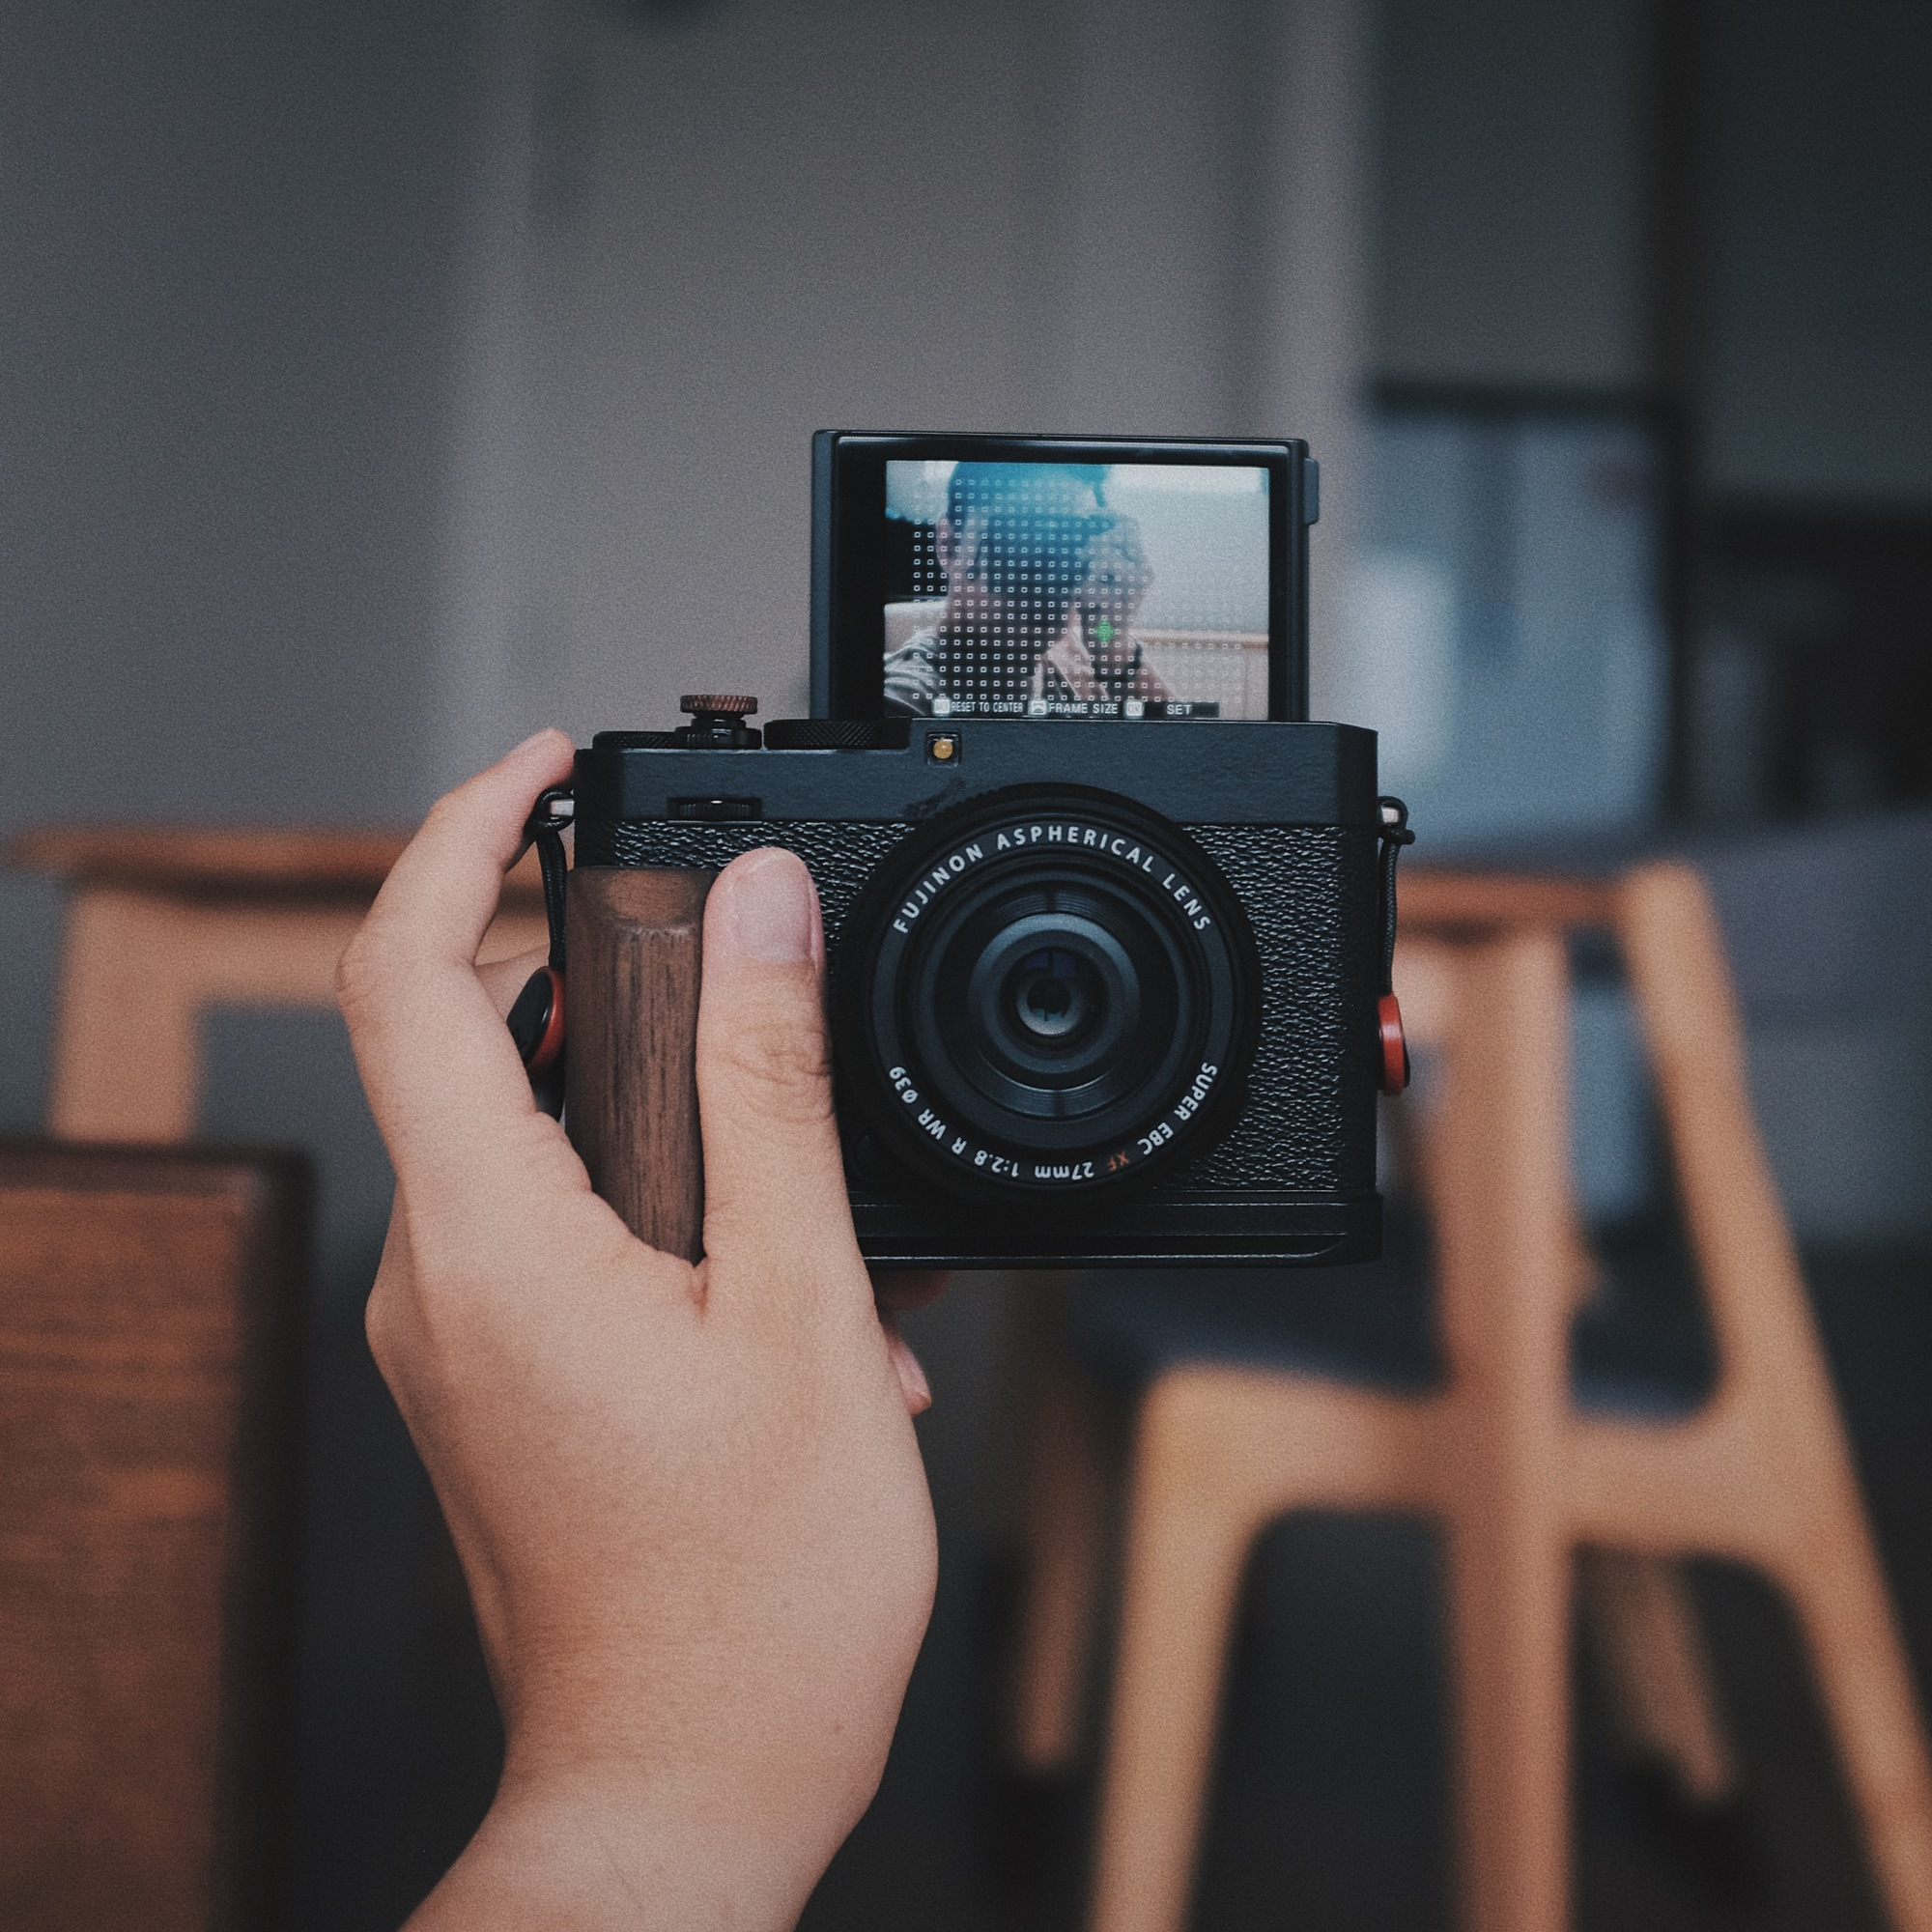
\includegraphics[width=\linewidth]{\envfinaldir/coverpic-prod.jpg}\par
            % \vskip 30pt
            \vfill

            \normalsize\rmfamily\scshape
            \copyright{} The Web Digest Project \hfill\large \envdatestr
        \end{center}
    \end{titlepage}
    % \restoregeometry
}
\newcommand{\simplehref}[1]{%
    \textcolor{blue!80!green}{\href{#1}{#1}}%
}
\renewcommand{\contentsname}{\center\Huge\sffamily\bfseries Contents\par\vskip 20pt}
\newcounter{ipartcounter}
\setcounter{ipartcounter}{0}
\newcommand{\ipart}[1]{
    % \vskip 20pt
    \clearpage
    \stepcounter{ipartcounter}
    \phantomsection
    \addcontentsline{toc}{chapter}{#1}
    % \begin{center}
    %     \Huge
    %     \sffamily\bfseries
    %     #1
    % \end{center}
    % \vskip 20pt plus 7pt
}
\newcounter{ichaptercounter}
\setcounter{ichaptercounter}{0}
\newcommand{\ichapter}[1]{
    % \vskip 20pt
    \clearpage
    \stepcounter{ichaptercounter}
    \phantomsection
    \addcontentsline{toc}{section}{\numberline{\arabic{ichaptercounter}}#1}
    \begin{center}
        \Huge
        \sffamily\bfseries
        #1
    \end{center}
    \vskip 20pt plus 7pt
}
\newcommand{\entrytitlefont}[1]{\subsection*{\raggedright\Large\sffamily\bfseries#1}}
\newcommand{\entryitemGeneric}[2]{
    % argv: title, url
    \parbox{\linewidth}{
        \entrytitlefont{#1}\par\vskip 5pt
        \footnotesize\ttfamily\mdseries
        \simplehref{#2}
    }\vskip 11pt plus 11pt minus 1pt
}
\newcommand{\entryitemGithub}[3]{
    % argv: title, url, desc
    \parbox{\linewidth}{
        \entrytitlefont{#1}\par\vskip 5pt
        \footnotesize\ttfamily\mdseries
        \simplehref{#2}\par\vskip 5pt
        \small\rmfamily\mdseries#3
    }\vskip 11pt plus 11pt minus 1pt
}
\newcommand{\entryitemAp}[3]{
    % argv: title, url, desc
    \parbox{\linewidth}{
        \entrytitlefont{#1}\par\vskip 5pt
        \footnotesize\ttfamily\mdseries
        \simplehref{#2}\par\vskip 5pt
        \small\rmfamily\mdseries#3
    }\vskip 11pt plus 11pt minus 1pt
}
\newcommand{\entryitemHackernews}[3]{
    % argv: title, hnurl, rawurl
    % \parbox{\linewidth}{
    %     \entrytitlefont{#1}\par\vskip 5pt
    %     \footnotesize\ttfamily\mdseries
    %     \simplehref{#3}\par
    %     \textcolor{black!50}{\href{#2}{#2}}
    % }\vskip 11pt plus 11pt minus 1pt
    \begin{minipage}{\linewidth}
            \entrytitlefont{#1}\par\vskip 5pt
            \footnotesize\ttfamily\mdseries
            \simplehref{#3}\par
            \textcolor{black!50}{\href{#2}{#2}}
    \end{minipage}\par\vskip 11pt plus 11pt minus 1pt
}







\begin{document}

\makeheader

\tableofcontents\clearpage




\ipart{Developers}
\ichapter{Hacker News}
\entryitemTwoLinks{Utah's hottest new power source is 15k feet below the ground}{https://news.ycombinator.com/item?id=45152569}{https://www.gatesnotes.com/utahs-hottest-new-power-source-is-below-the-ground}

\entryitemTwoLinks{How the "Kim" dump exposed North Korea's credential theft playbook}{https://news.ycombinator.com/item?id=45152066}{https://dti.domaintools.com/inside-the-kimsuky-leak-how-the-kim-dump-exposed-north-koreas-credential-theft-playbook/}

\entryitemTwoLinks{Zuckerberg Caught in Revealing Hot Mic Moment During White House Dinner}{https://news.ycombinator.com/item?id=45150759}{https://www.pcmag.com/news/zuckerberg-caught-in-revealing-hot-mic-moment-during-white-house-dinner}

\entryitemTwoLinks{Oldest recorded transaction}{https://news.ycombinator.com/item?id=45149626}{https://avi.im/blag/2025/oldest-txn/}

\entryitemTwoLinks{AI surveillance should be banned while there is still time}{https://news.ycombinator.com/item?id=45149281}{https://gabrielweinberg.com/p/ai-surveillance-should-be-banned}

\entryitemTwoLinks{996}{https://news.ycombinator.com/item?id=45149049}{https://lucumr.pocoo.org/2025/9/4/996/}

\entryitemTwoLinks{We hacked Burger King: How auth bypass led to drive-thru audio surveillance}{https://news.ycombinator.com/item?id=45148944}{https://bobdahacker.com/blog/rbi-hacked-drive-thrus/}

\entryitemTwoLinks{Qwen3 30B A3B Hits 13 token/s on 4xRaspberry Pi 5}{https://news.ycombinator.com/item?id=45148237}{https://github.com/b4rtaz/distributed-llama/discussions/255}

\entryitemTwoLinks{Let us git rid of it, angry GitHub users say of forced Copilot features}{https://news.ycombinator.com/item?id=45148167}{https://www.theregister.com/2025/09/05/github\_copilot\_complaints/}

\entryitemTwoLinks{Why language models hallucinate}{https://news.ycombinator.com/item?id=45147385}{https://openai.com/index/why-language-models-hallucinate/}

\entryitemTwoLinks{Rug pulls, forks, and open-source feudalism}{https://news.ycombinator.com/item?id=45146967}{https://lwn.net/SubscriberLink/1036465/e80ebbc4cee39bfb/}

\entryitemTwoLinks{GOP Cries Censorship Over Spam Filters That Work}{https://news.ycombinator.com/item?id=45146375}{https://krebsonsecurity.com/2025/09/gop-cries-censorship-over-spam-filters-that-work/}

\entryitemTwoLinks{Developing a Space Flight Simulator in Clojure}{https://news.ycombinator.com/item?id=45145794}{https://www.wedesoft.de/software/2025/09/05/clojure-game/}

\entryitemTwoLinks{A sunscreen scandal shocking Australia}{https://news.ycombinator.com/item?id=45145624}{https://www.bbc.com/news/articles/c4gzl41rpdqo}

\entryitemTwoLinks{GLM 4.5 with Claude Code}{https://news.ycombinator.com/item?id=45145457}{https://docs.z.ai/guides/llm/glm-4.5}

\entryitemTwoLinks{Tesla changes meaning of 'Full Self-Driving', gives up on promise of autonomy}{https://news.ycombinator.com/item?id=45144900}{https://electrek.co/2025/09/05/tesla-changes-meaning-full-self-driving-give-up-promise-autonomy/}

\entryitemTwoLinks{The Universe Within 12.5 Light Years}{https://news.ycombinator.com/item?id=45144337}{http://www.atlasoftheuniverse.com/12lys.html}

\entryitemTwoLinks{Kenvue stock drops on report RFK Jr will link autism to Tylenol during pregnancy}{https://news.ycombinator.com/item?id=45144123}{https://www.cnbc.com/2025/09/05/rfk-tylenol-autism-kenvue-stock-for-url.html}

\entryitemTwoLinks{Nest 1st gen and 2nd gen thermostats no longer supported from Oct 25}{https://news.ycombinator.com/item?id=45143879}{https://community.hubitat.com/t/nest-1st-gen-and-2nd-gen-thermostats-no-longer-supported-by-google-from-10-25-2025/152952}

\entryitemTwoLinks{I kissed comment culture goodbye}{https://news.ycombinator.com/item?id=45143077}{https://sustainableviews.substack.com/p/the-day-i-kissed-comment-culture}\ichapter{Phoronix}
\entryitemGeneric{\hskip 0pt{}Linux 6.17 Lands Fixes For Upcoming Rust 1.91}{https://www.phoronix.com/news/Linux-6.17-Rust-1.91}

\entryitemGeneric{\hskip 0pt{}Debian 13.1 Released With An Initial Batch Of Fixes}{https://www.phoronix.com/news/Debian-13.1-Released}

\entryitemGeneric{\hskip 0pt{}Rust Coreutils 0.2 Released With "Massive" Performance Gains, Production-Ready Ubuntu Support}{https://www.phoronix.com/news/Rust-Coreutils-0.2}

\entryitemGeneric{\hskip 0pt{}KDE Linux Enters Alpha As Reference Linux Distribution For The KDE Desktop}{https://www.phoronix.com/news/KDE-Linux-Alpha}

\entryitemGeneric{\hskip 0pt{}Linus Torvalds Grows Frustrated Seeing "Garbage" With "Link: " Tags In Git Commits}{https://www.phoronix.com/news/Linus-Torvalds-No-Link-Tags}

\entryitemGeneric{\hskip 0pt{}Linux 6.17 Merges Important Stability Fixes For Open-Source NVIDIA Driver}{https://www.phoronix.com/news/Linux-617-Better-Nouveau-Stable}

\entryitemGeneric{\hskip 0pt{}KDE Plasma 6.5 KWin Adding Support For GPU Underlays}{https://www.phoronix.com/news/KDE-Plasma-6.5-Underlays}

\entryitemGeneric{\hskip 0pt{}systemd 258 Closing In On Its Stable Release}{https://www.phoronix.com/news/systemd-258-rc4}

\entryitemGeneric{\hskip 0pt{}Pop!\_OS 24.04 Beta Along With COSMIC Desktop Beta In Late September}{https://www.phoronix.com/news/Pop-OS-24.04-COSMIC-Beta-Sep}


\ipart{Developers~~~~(zh-Hans)}
\ichapter{Solidot}
\entryitemGeneric{\hskip 0pt{}Google 因广告技术业务的反垄断行为被欧盟罚款 34.5 亿美元 }{https://www.solidot.org/story?sid=82239}

\entryitemGeneric{\hskip 0pt{}英国政府试用 M365 Copilot 后未发现明显的生产力提升}{https://www.solidot.org/story?sid=82238}

\entryitemGeneric{\hskip 0pt{}阿富汗地震已造成逾 3000 人死亡}{https://www.solidot.org/story?sid=82237}

\entryitemGeneric{\hskip 0pt{}Mark Zuckerberg 起诉 Mark Zuckerberg}{https://www.solidot.org/story?sid=82236}

\entryitemGeneric{\hskip 0pt{}上厕所时用智能手机大幅增加痔疮风险}{https://www.solidot.org/story?sid=82235}

\entryitemGeneric{\hskip 0pt{}人工甜味剂与认知能力下降相关,相当于衰老 1.6 年}{https://www.solidot.org/story?sid=82234}

\entryitemGeneric{\hskip 0pt{}Anthropic 禁止中国控股公司使用 Claude}{https://www.solidot.org/story?sid=82233}

\entryitemGeneric{\hskip 0pt{}尼泊尔屏蔽大部分社媒平台}{https://www.solidot.org/story?sid=82232}

\entryitemGeneric{\hskip 0pt{}微软开源 6502 BASIC }{https://www.solidot.org/story?sid=82231}

\entryitemGeneric{\hskip 0pt{}英特尔研发支出超英伟达和 AMD}{https://www.solidot.org/story?sid=82230}

\entryitemGeneric{\hskip 0pt{}Atlassian 以 6.1 亿美元收购 Browser Company  }{https://www.solidot.org/story?sid=82229}

\entryitemGeneric{\hskip 0pt{}美国失业人数超过招聘人数}{https://www.solidot.org/story?sid=82228}

\entryitemGeneric{\hskip 0pt{}Fina Root CA 签发了三张 1.1.1.1 证书}{https://www.solidot.org/story?sid=82227}

\entryitemGeneric{\hskip 0pt{}《空洞骑士:丝之歌》上线,各大游戏平台服务器全部崩溃}{https://www.solidot.org/story?sid=82226}

\entryitemGeneric{\hskip 0pt{}森林砍伐让亚马孙雨林旱季降雨减少}{https://www.solidot.org/story?sid=82225}

\entryitemGeneric{\hskip 0pt{}瑞士发布了完整开源的大模型 Apertus}{https://www.solidot.org/story?sid=82224}

\entryitemGeneric{\hskip 0pt{}研究预测地球碳封存能力上限为 1.46 万亿吨}{https://www.solidot.org/story?sid=82223}

\entryitemGeneric{\hskip 0pt{}美国撤销台积电南京工厂的优待措施}{https://www.solidot.org/story?sid=82222}

\entryitemGeneric{\hskip 0pt{}照亮微塑料的细菌}{https://www.solidot.org/story?sid=82221}

\entryitemGeneric{\hskip 0pt{}太阳耀斑温度比以前认为的高出 6.5 倍}{https://www.solidot.org/story?sid=82220}\ichapter{V2EX}
\entryitemGeneric{\hskip 0pt{}[生活] 小孩马上满一岁了,想给孩子买保险,各位大哥有啥建议或者要避开的坑不,求指导}{https://www.v2ex.com/t/1157562}

\entryitemGeneric{\hskip 0pt{}[分享创造] AI 女友迭代第二弹}{https://www.v2ex.com/t/1157561}

\entryitemGeneric{\hskip 0pt{}[生活] 我爸冠心病,一个月后要放支架,请问现在买什么保险能享受报销?}{https://www.v2ex.com/t/1157560}

\entryitemGeneric{\hskip 0pt{}[Google] 那个谷歌安全码是什么使用逻辑?}{https://www.v2ex.com/t/1157559}

\entryitemGeneric{\hskip 0pt{}[问与答] vscode ssh 连接新服务器的时候,有没有办法自动安装一些我指定的插件?}{https://www.v2ex.com/t/1157558}

\entryitemGeneric{\hskip 0pt{}[iPhone] 群晖 nas 能代替 icloud 吗}{https://www.v2ex.com/t/1157557}

\entryitemGeneric{\hskip 0pt{}[分享创造] Nano Banana 的羊毛也是给我蹭上了}{https://www.v2ex.com/t/1157555}

\entryitemGeneric{\hskip 0pt{}[推广] 上线一个有点意思的小站: https://ai-miniatur.org/}{https://www.v2ex.com/t/1157554}

\entryitemGeneric{\hskip 0pt{}[职场话题] 看了这么多篇论述什么后端已死切图仔已死}{https://www.v2ex.com/t/1157551}

\entryitemGeneric{\hskip 0pt{}[分享创造] 现在才做 Nano Banana 这个词是不是有点晚了}{https://www.v2ex.com/t/1157550}

\entryitemGeneric{\hskip 0pt{}[问与答] 突然发现英式早餐好像很有道理.}{https://www.v2ex.com/t/1157549}

\entryitemGeneric{\hskip 0pt{}[宽带症候群] GoDNS v3.3 发布: DDNS 客户端新增多服务商管理}{https://www.v2ex.com/t/1157548}

\entryitemGeneric{\hskip 0pt{}[Python] 在爬一些数据,如果请求过于频繁,其实也不是特别频繁,容易被 ip 封禁,有啥好用的免费 ip 池吗?或者付费的也行}{https://www.v2ex.com/t/1157547}

\entryitemGeneric{\hskip 0pt{}[Android] 大家通过 Android 系统级途径分享图片到 8.0.62 版本的微信会出现问题吗?}{https://www.v2ex.com/t/1157546}

\entryitemGeneric{\hskip 0pt{}[问与答] 有没有可以在 Android 上离线跑的语音识别模型?}{https://www.v2ex.com/t/1157545}

\entryitemGeneric{\hskip 0pt{}[Apple] 开发了一款``比较智能''的苹果相册 APP,可以文搜图或者按人脸和地点快速查找照片}{https://www.v2ex.com/t/1157544}

\entryitemGeneric{\hskip 0pt{}[问与答] 想了解下 台湾那边的半导体资讯网 哪个比较准 而且消息的时效性比较快?}{https://www.v2ex.com/t/1157543}

\entryitemGeneric{\hskip 0pt{}[问与答] 求推荐 2000 元左右安卓机}{https://www.v2ex.com/t/1157541}

\entryitemGeneric{\hskip 0pt{}[Apple] 土区 iCloud 转到国区,家庭组需要解散重组吗}{https://www.v2ex.com/t/1157540}

\entryitemGeneric{\hskip 0pt{}[问与答] 朋友们, 请问我通过淘宝或者京东的 api 做一个自己的电商 App 吗?}{https://www.v2ex.com/t/1157539}

\entryitemGeneric{\hskip 0pt{}[问与答] ShardingSphere 分表是否支持 standard 和 hint 同时使用?任务需要依次遍历所有分表}{https://www.v2ex.com/t/1157538}

\entryitemGeneric{\hskip 0pt{}[投资] 有没有比较稳定的股市行情数据啊,不用实时的}{https://www.v2ex.com/t/1157537}

\entryitemGeneric{\hskip 0pt{}[分享创造] 独立数字音乐作者 // Independent Digital Musician}{https://www.v2ex.com/t/1157536}

\entryitemGeneric{\hskip 0pt{}[硬件] 求游戏本推荐}{https://www.v2ex.com/t/1157535}

\entryitemGeneric{\hskip 0pt{}[问与答] [不懂就问] 截止发帖时间, 当前最好用的 AI 模型是哪个?请推荐}{https://www.v2ex.com/t/1157534}

\entryitemGeneric{\hskip 0pt{}[问与答] [求职碎碎念]入职第一天被拉去救火,组员凌晨还在群里讨论工作,所以光速跑路了}{https://www.v2ex.com/t/1157532}

\entryitemGeneric{\hskip 0pt{}[推广] 用免费的 CLI 写代码感觉还可以,不是打广告}{https://www.v2ex.com/t/1157531}

\entryitemGeneric{\hskip 0pt{}[程序员] Web 缓存网升级 CDNJS 加速服务啦!}{https://www.v2ex.com/t/1157530}

\entryitemGeneric{\hskip 0pt{}[程序员] 试用 codex 感想:不说 You are absolutely right 是 GPT-5 最好的编程特性之一}{https://www.v2ex.com/t/1157529}

\entryitemGeneric{\hskip 0pt{}[职场话题] 前端死没死不清楚,我们公司的前端马上死了}{https://www.v2ex.com/t/1157528}

\entryitemGeneric{\hskip 0pt{}[程序员] 有 Chrome 无损迁移的工具吗?}{https://www.v2ex.com/t/1157526}

\entryitemGeneric{\hskip 0pt{}[问与答] 我想把自己开发的应用推广到海外市场,但是不想付广告费,在 Reddit 发帖是一个好方案吗?}{https://www.v2ex.com/t/1157525}

\entryitemGeneric{\hskip 0pt{}[问与答] 问下 USB 延长线对电压、电流和输出功率的影响}{https://www.v2ex.com/t/1157524}

\entryitemGeneric{\hskip 0pt{}[硬件] 暗影精灵 11,华硕天选 6pro,联想 y7000p 哪个好点?}{https://www.v2ex.com/t/1157523}

\entryitemGeneric{\hskip 0pt{}[生活] 小孩寻死觅活要辞职公务员,求如何让他回心转意?}{https://www.v2ex.com/t/1157522}

\entryitemGeneric{\hskip 0pt{}[分享创造] 我们恰好做了开源版本 Claude for Chrome (浏览器自动化)}{https://www.v2ex.com/t/1157518}

\entryitemGeneric{\hskip 0pt{}[职场话题] 要接受大疆的 offer 么?}{https://www.v2ex.com/t/1157517}

\entryitemGeneric{\hskip 0pt{}[问与答] 想问问大家 iPad 都是怎么看 epub 格式的书,苹果自带的图书好像打开不了一些第三方的书?}{https://www.v2ex.com/t/1157516}

\entryitemGeneric{\hskip 0pt{}[问与答] 被玻璃自爆伤害,应该由谁承担责任?}{https://www.v2ex.com/t/1157515}

\entryitemGeneric{\hskip 0pt{}[生活] 招商银行牛逼\&有什么好看的卡吗}{https://www.v2ex.com/t/1157514}

\entryitemGeneric{\hskip 0pt{}[Solana] 回测数据可以去哪里获取?}{https://www.v2ex.com/t/1157513}

\entryitemGeneric{\hskip 0pt{}[问与答] 大佬们有没有好用的 ClaudeCode 中转推荐一下,稳定一些的}{https://www.v2ex.com/t/1157512}

\entryitemGeneric{\hskip 0pt{}[程序员] 我的塑料盒子机箱}{https://www.v2ex.com/t/1157509}

\entryitemGeneric{\hskip 0pt{}[酷工作] 高级前端开发}{https://www.v2ex.com/t/1157508}

\entryitemGeneric{\hskip 0pt{}[问与答] 图形评测题答案讨论}{https://www.v2ex.com/t/1157506}

\entryitemGeneric{\hskip 0pt{}[硬件] [求助赛博神医] 为什么我的电脑在打开网页时出现谜之马赛克?我该怎么排查问题}{https://www.v2ex.com/t/1157505}

\entryitemGeneric{\hskip 0pt{}[程序员] chromium 代码中的 Profile 概念有点复杂呀}{https://www.v2ex.com/t/1157503}

\entryitemGeneric{\hskip 0pt{}[问与答] 网络安全 CTF 竞赛用什么 LLM 合适?}{https://www.v2ex.com/t/1157502}

\entryitemGeneric{\hskip 0pt{}[路由器] 各位 V2EXer 大佬们,小弟新房装修,有一些家庭网络规划(路由器选择、网络拓扑、点位布置、弱电箱散热)相关的问题想要请教}{https://www.v2ex.com/t/1157501}

\entryitemGeneric{\hskip 0pt{}[分享创造] 国内有玩 Wplace 这个游戏的朋友吗?欢迎免费试用提意见}{https://www.v2ex.com/t/1157500}


\ipart{Generic News}







\clearpage
\leavevmode\vfill
\footnotesize

Copyright \copyright{} 2023-2025 Neruthes and other contributors.

This document is published with CC BY-NC-ND 4.0 license.

The entries listed in this newsletter may be copyrighted by their respective creators.

This newsletter is generated by the Web Digest project.

The newsletters are also delivered via Telegram channel \CJKunderline{\href{https://t.me/webdigestchannel}{https://t.me/webdigestchannel}}.\\
RSS feed is available at \CJKunderline{\href{https://webdigest.pages.dev/rss.xml}{https://webdigest.pages.dev/rss.xml}}.

This newsletter is available in PDF at
\CJKunderline{\href{https://webdigest.pages.dev/}{https://webdigest.pages.dev/}}.

The source code being used to generate this newsletter is available at\\
\CJKunderline{\href{https://github.com/neruthes/webdigest}{https://github.com/neruthes/webdigest}}.

This newsletter is also available in
\CJKunderline{\href{http://webdigest.pages.dev/readhtml/\envyear/WebDigest-20250907.html}{HTML}} and
\CJKunderline{\href{https://github.com/neruthes/webdigest/blob/master/markdown/\envyear/WebDigest-20250907.md}{Markdown}}.


\coverpic{https://unsplash.com/photos/winding-hiking-trail-through-grassy-mountainside-with-trees-G\_w2LWtxp-4}{Emma Swoboda}


\end{document}
